\section{Experiments}

\subsection{Settings}
\paragraph{Datasets}
To comprehensively assess the effectiveness of compressed prompts in retaining LLM abilities, we evaluated their performance across four datasets.
For reasoning and in-context learning (ICL), we use \textbf{GSM8K}~\cite{cobbe2021training} and \textbf{BBH}~\cite{suzgun2022challenging}.
% for question answering and 
As for contextual understanding, we use \textbf{ShareGPT}~\cite{sharegpt} for conversation and \textbf{Arxiv-March23}~\cite{li2023unlocking} for summarization.
% It is worth mentioning that none of these evaluation datasets have been seen by either the small LM or the target LLMs, particularly the latter two datasets, which were newly collected this year.
It's worth noting that neither the small LM nor the target LLMs used in this paper have seen any of the evaluation datasets, especially the last two which were newly collected this year.
We followed the experimental setup of previous work~\cite{fu2023chain,li2023unlocking} for the usage of these datasets.
Please refer to Appendix~\ref{sec:dataset_detail} for detailed information.
% Detailed information can be found in the Appendix~\ref{sec:dataset_detail}.


\paragraph{Evaluation}
Following \citet{cobbe2021training}, \citet{fu2023chain}, and \citet{li2023unlocking}, we utilize the Exact Match as the evaluation metric for GSM8K and BBH.
We use BLEU~\cite{papineni2002bleu}, ROUGE~\cite{lin2004rouge}, and BERTScore~\cite{zhang2020BERTScore} as the evaluation metrics for ShareGPT and Arxiv-March23.

\paragraph{Implementation Details}
In this paper, we employ the GPT-3.5-Turbo-0301 and the Claude-v1.3 %variant of the powerful models 
as the target LLMs, which can be accessed via OpenAI\footnote{https://platform.openai.com/} and Claude API\footnote{https://anthropic.com/}.
% To achieve more stable outputs from LLMs,
To improve the stability of outputs produced by LLMs
we apply greedy decoding with a temperature of $0$ across all experiments.
% set the decoding temperature to $0$.
% and top $p$ to $1$.
% We only use the Alpaca dataset~\cite{alpaca} to align the small language models with black-box LLMs, and it is not involved in the evaluation process.
The Alpaca dataset~\cite{alpaca} is exclusively employed for aligning small language models with black-box LLMs, and is not utilized in the evaluation process. 
In our experiments, we utilize either Alpaca-7B\footnote{https://github.com/tatsu-lab/stanford\_alpaca} or GPT2-Alpaca as the small pre-trained language model $\mathcal{M}_s$ for compression.
% For the small pre-trained langauge model $\mathcal{M}_s$, we utilize the Alpaca-7B\footnote{https://github.com/tatsu-lab/stanford\_alpaca} and the GPT2-Alpaca.
We implement our approach based on PyTorch 1.12.0\footnote{https://pytorch.org/} and Huggingface's Transformers\footnote{https://github.com/huggingface/transformers}.
We set the granular control coefficient $k$ to $2$.
We use the pre-defined compression rates $\tau_{\text{ins}}=0.85$ and $\tau_{\text{que}}=0.9$ for instructions and questions.
The segment size used in the iterative token-level compression is set to $100$.

\begin{table*}[!ht]
    \centering
    \setlength{\tabcolsep}{1mm}
    \vspace{-2ex}
    \resizebox{2\columnwidth}{!}{
    \begin{tabular}{l|ccccccc|ccccccc}
    \toprule
        \multirow{2}{*}{Methods} &  \multicolumn{7}{@{}c}{{\bf ShareGPT}} &  \multicolumn{7}{@{}c}{{\bf Arxiv-March23}} \\
        & BLEU & Rouge1 & Rouge2 & RougeL & BS F1 & Tokens & $1/\tau$ & BLEU & Rouge1 & Rouge2 & RougeL & BS F1 & Tokens & $1/\tau$\\
        % \hline
         \cmidrule (r){1-1}\cmidrule (lr){2-8} \cmidrule (lr){9-15}
     \multicolumn{1}{@{}l}{{\bf \textit{Constraint I}}} & \multicolumn{7}{@{}l}{{ \textit{2x constraint}}} & \multicolumn{7}{@{}l}{{ \textit{350 tokens constraint}}}  \\ 
    Sentence Selection & \textbf{28.59} & 46.11 & \textbf{31.07} & 37.94 & 88.64 & 388 & 1.5x & 22.77 & 50.1 & 25.93 & 33.63 & 88.21 & 379 & 4x \\
    Selective-Context & 25.42 & 46.47 & 29.09 & 36.99 & 88.92 & 307 & 1.9x & 21.41 & 51.3 & 27.94 & 36.73 & 89.60 & 356 & 4x \\
    % GPT4 Generation & 71.87 & 496 & 5x \\
    {\cellcolor[rgb]{0.925,0.957,1}}\textbf{Ours} & {\cellcolor[rgb]{0.925,0.957,1}}27.36 & {\cellcolor[rgb]{0.925,0.957,1}}\textbf{48.87} & {\cellcolor[rgb]{0.925,0.957,1}}30.32 & {\cellcolor[rgb]{0.925,0.957,1}}\textbf{38.55} & {\cellcolor[rgb]{0.925,0.957,1}}\textbf{89.52} &{\cellcolor[rgb]{0.925,0.957,1}}304 & {\cellcolor[rgb]{0.925,0.957,1}}1.9x  & {\cellcolor[rgb]{0.925,0.957,1}}\textbf{23.15} & {\cellcolor[rgb]{0.925,0.957,1}}\textbf{54.21} & {\cellcolor[rgb]{0.925,0.957,1}}\textbf{32.66} & {\cellcolor[rgb]{0.925,0.957,1}}\textbf{42.74} & {\cellcolor[rgb]{0.925,0.957,1}}\textbf{90.33} & {\cellcolor[rgb]{0.925,0.957,1}}345 & {\cellcolor[rgb]{0.925,0.957,1}}4x \\
     \hline
     \hline
     \multicolumn{1}{@{}l}{{\bf \textit{Constraint II}}} & \multicolumn{7}{@{}l}{{ \textit{3x constraint}}} & \multicolumn{7}{@{}l}{{ \textit{175 tokens constraint}}}  \\ 
    Sentence Selection & 18.94 & 35.17 & 18.96 & 26.75 & 85.63 & 255 & 2.3x & 12.41 & 38.91 & 14.25 & 26.72 & 87.09 & 229 & 7x \\
    Selective-Context & 15.79 & 38.42 & 20.55 & 28.89 & 87.12 & 180 & 3.3x & 12.23 & 42.47 & 19.48 & 29.47 & 88.16 & 185 & 8x\\
    {\cellcolor[rgb]{0.925,0.957,1}}\textbf{Ours} & {\cellcolor[rgb]{0.925,0.957,1}}\textbf{19.55} & {\cellcolor[rgb]{0.925,0.957,1}}\textbf{40.81} & {\cellcolor[rgb]{0.925,0.957,1}}\textbf{22.68} & {\cellcolor[rgb]{0.925,0.957,1}}\textbf{30.98} & {\cellcolor[rgb]{0.925,0.957,1}}\textbf{87.70} &{\cellcolor[rgb]{0.925,0.957,1}}177 & {\cellcolor[rgb]{0.925,0.957,1}}3.3x & {\cellcolor[rgb]{0.925,0.957,1}}\textbf{13.45} & {\cellcolor[rgb]{0.925,0.957,1}}\textbf{44.36} & {\cellcolor[rgb]{0.925,0.957,1}}\textbf{24.86} & {\cellcolor[rgb]{0.925,0.957,1}}\textbf{34.94} & {\cellcolor[rgb]{0.925,0.957,1}}\textbf{89.03} & {\cellcolor[rgb]{0.925,0.957,1}}176 & {\cellcolor[rgb]{0.925,0.957,1}}9x \\
    \bottomrule
    \end{tabular}
    }
    \caption{Performance of different methods under different target compression ratios on the conversation (ShareGPT) and summarization (Arxiv-March23) task.}
    \label{tab:main_results_context}
\end{table*}



\begin{table}[tb]
    \centering
    \setlength{\tabcolsep}{1mm}
    \vspace{-2ex}
    \resizebox{1\columnwidth}{!}{
    \begin{tabular}{l|ccc|ccc}
    \toprule
        \multirow{2}{*}{Methods} &  \multicolumn{3}{@{}c}{{\bf GSM8K}} &  \multicolumn{3}{@{}c}{{\bf BBH}} \\
         & EM & Tokens & $1/\tau$ & EM & Tokens & $1/\tau$\\
        % \hline
         \cmidrule (r){1-1}\cmidrule (lr){2-4} \cmidrule (lr){5-7}
     Full-shot & 78.85 & 2,366 & - & 70.07 & 774 & -  \\
     \hline
     \hline
     \multicolumn{4}{@{}l}{{\bf \textit{1-shot constraint}}} \\ 
    1-shot & 77.10 & 422 & 6x & 69.60 & 284 & 3x \\
    Selective-Context & 53.98 & 452 & 5x & 54.27 & 276 & 3x \\
    GPT4 Generation & 71.87 & 496 & 5x & 27.13 & 260 & 3x \\
    {\cellcolor[rgb]{0.925,0.957,1}}\textbf{Ours} & {\cellcolor[rgb]{0.925,0.957,1}}\textbf{79.08} & {\cellcolor[rgb]{0.925,0.957,1}}446 & {\cellcolor[rgb]{0.925,0.957,1}}5x & {\cellcolor[rgb]{0.925,0.957,1}}\textbf{70.11} & {\cellcolor[rgb]{0.925,0.957,1}}288 & {\cellcolor[rgb]{0.925,0.957,1}}3x \\
     \hline
     \hline
     \multicolumn{4}{@{}l}{{\bf \textit{half-shot constraint}}} \\ 
    Sentence Selection & 72.33 & 230 & 10x & 39.56 & 175 & 4x\\
    Selective-Context & 52.99 & 218 & 11x & 54.02 & 155 & 5x \\
    GPT4 Generation & 68.61 & 223 & 11x & 27.09 & 161 & 5x \\
    {\cellcolor[rgb]{0.925,0.957,1}}\textbf{Ours} & {\cellcolor[rgb]{0.925,0.957,1}}\textbf{77.41} & {\cellcolor[rgb]{0.925,0.957,1}}171 & {\cellcolor[rgb]{0.925,0.957,1}}14x & {\cellcolor[rgb]{0.925,0.957,1}}\textbf{61.60} & {\cellcolor[rgb]{0.925,0.957,1}}171 & {\cellcolor[rgb]{0.925,0.957,1}}5x \\
     \hline
     \hline
     \multicolumn{4}{@{}l}{{\bf \textit{quarter-shot constraint}}} \\ 
    Sentence Selection & 66.67 & 195 & 12x & 46.00 & 109 & 7x \\
    Selective-Context & 44.20 & 157 & 15x & 47.37 & 108 & 7x \\
    GPT4 Generation & 56.33 & 188 & 20x & 26.81 & 101 & 8x \\
    {\cellcolor[rgb]{0.925,0.957,1}}\textbf{Ours} & {\cellcolor[rgb]{0.925,0.957,1}}\textbf{77.33} & {\cellcolor[rgb]{0.925,0.957,1}}117 & {\cellcolor[rgb]{0.925,0.957,1}}20x & {\cellcolor[rgb]{0.925,0.957,1}}\textbf{56.85} & {\cellcolor[rgb]{0.925,0.957,1}}110 & {\cellcolor[rgb]{0.925,0.957,1}}7x \\
     \hline
     \hline
    zero-shot & 48.75$^{\dag}$ & 11 & 215x & 32.32 & 16 & 48x \\
    Simple Prompt & 74.9 & 691 & 3x & - & - & - \\
    \bottomrule
    \end{tabular}
    }
    \caption{Performance of different methods under different target compression ratios on the GSM8K mathematical reasoning and Big-bench Hard (BBH) datasets. $^{\dag}$We also include the instruction of the prompt in zero-shot experiments for a vertical comparison.}
    \label{tab:main_results}
\end{table}

\paragraph{Baselines}
We consider the following baselines:
\begin{itemize}
\setlength{\itemsep}{0pt}
\item \textit{GPT4-Generation}: Instruct GPT-4 to compress the original prompt.
% \red{
% We utilize various instructions to guide GPT-4 in compressing the prompt, and select the best result as the final outcome. 
We used ten sets of instructions here and reported the best results.
Appendix~\ref{sec:gpt4_generation_instructions} displays the instructions we employed.
\item \textit{Random Selection}: Random select the demonstrations or sentences of the original prompt.
\item \textit{Selective-Context} \cite{li2023unlocking}: Use the phrase-level self-information from a small language model to filter out less informative content. We use the same small LM, \ie, Alpaca-7B for a fair comparison.
\end{itemize}

\subsection{Main Results}
% 大表 GSM8K, BBH, CHAT, SUmmarization

Table~\ref{tab:main_results_context} and \ref{tab:main_results} report the results of our approach alongside those baseline methods % in difference compression constraint
on GSM8K, BBH, ShareGPT, and Arxiv-March23.
It can be seen that our proposed method consistently outperforms the prior methods by a large margin in almost all experiments.

Specifically, on GSM8K and BBH, the reasoning and in-context learning-related benchmark, our method even achieves slightly higher results than the full-shot approach, while also delivering impressive compression ratios ($1 / \tau$) of 5x and 3x respectively, with the 1-shot constraint.
This well demonstrates that our compressed prompts effectively retain the reasoning information contained in the original prompt.
As the compression ratio increases, \ie, under the half-shot and quarter-shot constraints, the performance experiences a slight decline.
For instance, on GSM8K, the EM scores will decrease by 1.44 and 1.52, respectively, despite compression ratios as high as 14x and 20x.
On BBH, our approach achieves compression ratios of 5x and 7x with the EM score decreasing by 8.5 and 13.2 points, respectively.
% \textcolor{red}{
% which is close to the performance of PaLM-540B at 62.0.
In fact, this performance is already quite satisfactory, as it approaches the score of 62.0 achieved by PaLM-540B in half-shot constraint.
% } 
Our case study reveals that this declined performance on BBH is mainly due to challenging reasoning tasks, such as tracking\_shuffled\_objects\_seven\_objects.

Moreover, on ShareGPT and Arxiv-March23, two contextual understanding benchmarks, we can see that
our approach achieves acceleration ratios of 9x and 3.3x with a high BERTScore F1, indicating that our approach successfully retains the semantic information of the initial prompts. % This will help save substantial computation and cost in various long prompt scenarios.
% that BERTScore F1 across multiple compression ratios consistently lie in the range from 88 to 90, indicating that our approach successfully retains the semantic information of the initial prompts.
% \textcolor{red}{Our method outperforms baselines across most compression ratios, especially selective-context, with BERTScore F1 values superior by 0.6 and 0.58, 0.73 and 0.87 for ShareGPT and Arxiv, respectively. This is because phrase-level self-information does not consider the conditional non-independence between tokens, leading to the loss of some critical information. Our approach achieves acceleration ratios of 9x and 3.3x in summarization and conversation tasks, respectively, with only a slight performance loss. This will help save substantial computation and cost in various long prompt scenarios.}

\subsection{Analysis on Reasoning \& ICL Tasks.}
Here we analyze the performance of our approach and baseline methods on the difficult reasoning and in-context learning (ICL) benchmarks GSM8K and BBH.
% Particularly, on GSM8K, our method achieves up to \textbf{20x} compression ratio with only a \textbf{1.52}-point performance loss. These results demonstrate the effectiveness of the proposed approach.
% % achieving a  performance of up to 20x compress ratio with only 1.52 points drop on GSM8K. This well demonstrates the effectiveness of the proposed approach.

% \paragraph{GSM8K \& BBH} 
% Table \ref{tab:main_results} shows how the compressed prompts perform on the reasoning and in-context learning tasks.
% % We utilize GSM8K and BBH two hard reseaoning tasks to evaluate the reasoning and ICL capacity of the compressed prompts.
% We can see that our compressed prompts effectively retain the reasoning information contained in the original prompt.
% % As observed, our method effectively retains the reasoning information within the prompt.


% Under the setting of the 1-shot constraint, our method even achieves slightly higher results than the full-shot approach, while also delivering impressive compression ratios ($1 / \tau$) of 5x and 3x on GSM8K and BBH, respectively.
% As the compression ratio increases, the performance experiences a slight decline.
% For instance, on GSM8K, % with 14x and 20x compression ratios, the EM scores decrease by 1.44 and 1.52, respectively.
% when compressing 14x and 20x, the EM scores will decrease by 1.44 and 1.52, respectively.
% % In BBH, the EM scores decrease by 9.3 and 13.9 with 5x and 7x compression ratios, respectively, % 
% % which is close to the performance of PaLM-540B at 62.0. 
% % achieves competitive performance with PaLM-540B
% On BBH, our approach achieves compression ratios of 5x and 7x which the EM score decreasing by 8.5 and 13.2 points when subjected to half-shot constraint and quarter-shot constraint, respectively, \textcolor{red}{which is close to the performance of PaLM-540B at 62.0.} 
% Our case study reveals that this declined performance on BBH is mainly due to challenging reasoning tasks, such as tracking\_shuffled\_objects\_seven\_objects.

We notice that our approach shows significant performance improvements over the strong baseline Selective-Context under all settings. 
% Still, our approach shows significant performance improvements when compared to other baseline methods, such as the strong \textit{selective-context}. %, especially for the strong baseline selective-context.
% It is evident that the phrase token-level self-information method 
We conjecture that,
% the \textit{Selective-Context} method, which relies on phrase-level self-information, 
as relying on phrase-level self-information, Selective-Context is prone to lose critical reasoning information during the chain-of-thought process. 
Especially on GSM8K, its performance is lower than ours by 33.10 points at a compression ratio of 20x. % compression ratio, the performance drops by 33.10 compared to ours.
The inferior performance of Sentence Selection suggests that it may face similar issues of fragmentary reasoning logic.
% Sentence Selection faces similar issues, especially when dealing with multi-step chain-of-thought prompts in GSM8K. 
% Its inferior performance also suggests that it may be missing important reasoning steps and suffering from incomplete reasoning logic.
Surprisingly, though GPT-4 has demonstrated its strong text generation capability, the suboptimal performance on prompt compression indicates that the generated prompts may omit crucial details from the original prompt, particularly reasoning steps. 
% As a result, its performance in reasoning tasks is generally suboptimal.

In addition to the findings mentioned above,
the experiments also demonstrate that our method can preserve the ICL capacity of prompts for LLMs.
Compared to the zero-shot results, our approach exhibits significant performance improvements of 51.55 and 24.53 even with the largest compression ratios.
Notably, on GSM8K, our 20x compressed prompt outperforms the 8-shot 3-step CoT by 2.43, further suggesting that our method can effectively retain the reasoning information.

% \paragraph{Contextual Understanding}
% \paragraph{ShareGPT \& Arxiv-March23}
% Table~\ref{tab:main_results_context} shows the results on contextual understanding tasks. 
% % Table~\ref{tab:main_results_context} shows the results for ShareGPT and Arxiv. 
% % Our method effectively preserves the semantic information of the original prompts at various compression ratios, with BERTScore F1 consistently ranging from 88 to 90.
% We can see that BERTScore F1 points across multiple compression ratios consistently lie in the range from 88 to 90, indicating that our approach successfully retains the semantic information of the initial prompts.
% \textcolor{red}{Although traditional n-gram evaluation metrics, particularly BLEU, exhibit a significant drop, they do not adequately reflect the actual generation performance of compressed prompts due to the uncontrollable generation content of complex LLMs.}


% \textcolor{red}{Our method outperforms baselines across most compression ratios, especially selective-context, with BERTScore F1 values superior by 0.6 and 0.58, 0.73 and 0.87 for ShareGPT and Arxiv, respectively. This is because phrase-level self-information does not consider the conditional non-independence between tokens, leading to the loss of some critical information. Our approach achieves acceleration ratios of 9x and 3.3x in summarization and conversation tasks, respectively, with only a slight performance loss. This will help save substantial computation and cost in various long prompt scenarios.}

\subsection{Ablation}
To validate the contributions of different components in our approach, we introduce five variants of our model for ablation study:
i) \textit{Ours w/o Iterative Token-level Compression}, which performs token-level compression in a single inference rather than iteratively.
ii) \textit{Ours w/o Budget Controller}, which directly employs ITPC with the same compression ratio for all components.
iii) \textit{Ours w/o Dynamic Compression Ratio}, which uses the same compression ratio for all components.
iv) \textit{Ours w/ Random Selection in Budget Controller}, which randomly selects demonstrations or sentences for demonstration-level prompt compression.
v) \textit{Ours w/o Distribution Alignment}, which removes the distribution alignment module of our approach and directly use the pre-trained LLaMA-7B as the small language model.
% relies on a non-alignment model, such as LLaMA-7B, as the small LM.
vi) \textit{Ours w/ Remove Stop Words}, which removes the stop words in original prompts using NLTK\footnote{https://www.nltk.org/}.
Table~\ref{tab:ablation} shows the results.
\begin{figure}[t]
    \centering
    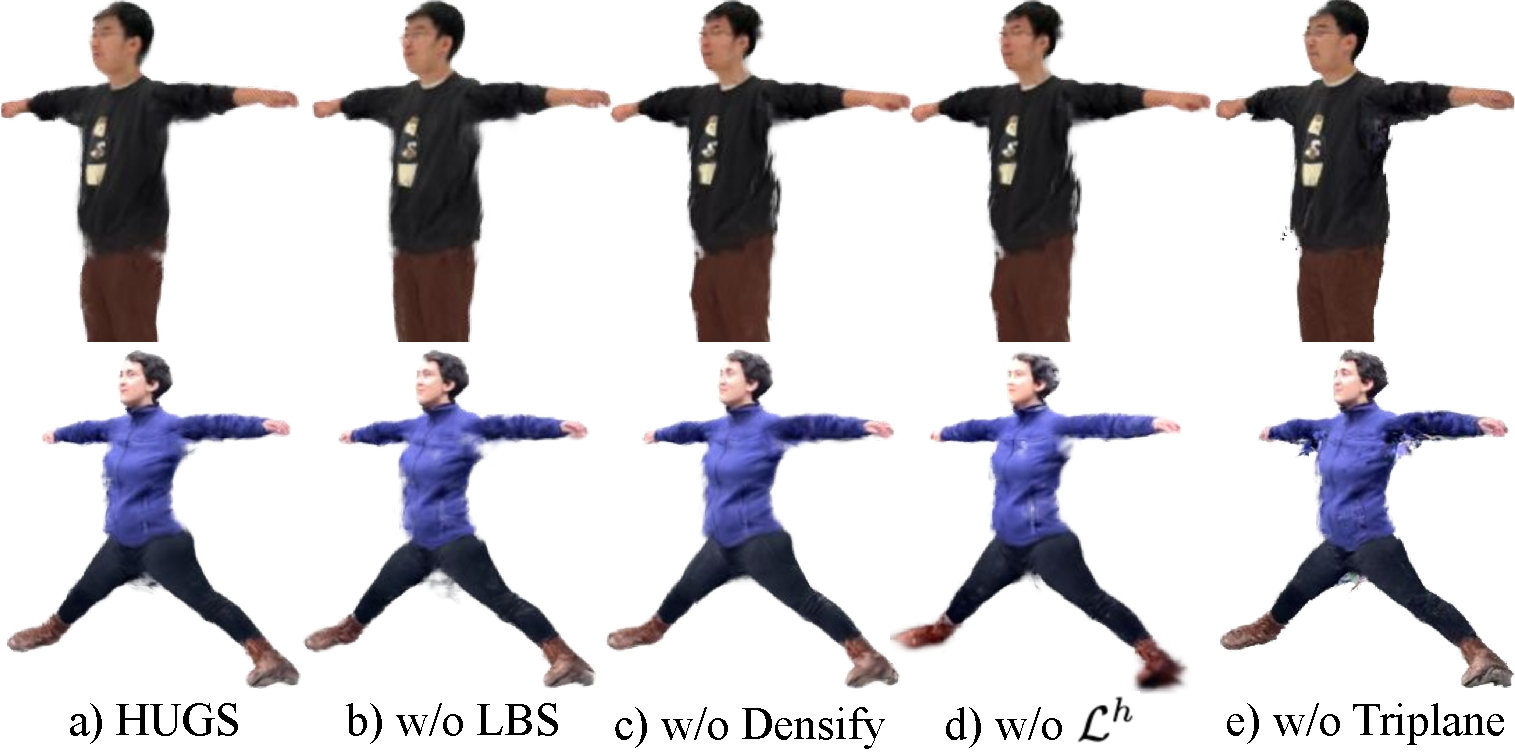
\includegraphics[width=\linewidth]{figures/pdf_files/ablation_qual.pdf}
    % \begin{tabular}{cc}
    %      NeuMan~\cite{jiang2022neuman} \quad \quad & \qquad \qquad HUGS (ours) 
    % \end{tabular}
    \caption{\textbf{Ablation study} showing the visualization of details captured in the human canonical shape under different ablations of our method.} 
    \label{fig:ablation}
\end{figure}

Comparing Ours with w/o Iterative Token-level Prompt Compression, we observe a significant decline in Exact Match when the conditional dependence between compressed tokens is not considered.
We conjecture this variant may lose essential information in the prompt, especially for low-frequency keywords that frequently appear in the given prompt.
When comparing Ours with w/o Dynamic Compression Ratio and with w/o Budget Controller, it reveals that different components of the prompt exhibit varying sensitivity.
Instructions and questions necessitate a lower compression ratio.
To balance the relationship between compression ratio and language integrity, introducing a demonstration or sentence-level filter better preserves sufficient linguistic information, even at higher compression ratios. Ours w/ Random Selection in Budget Controller indicates that selecting sentences or demonstrations based on perplexity can better identify information-rich sentences for target LLMs.
Distribution Alignment allows small LMs to generate distributions that more closely resemble those of target LLMs, resulting in a further improvement of 0.56 on GSM8K.


\subsection{Discussion}

\paragraph{Different Target LLMs}
Here we test our method with Claude-v1.3 as the target LLM to demonstrate its generalizability across different black-box LLMs in addition to the GPT series models. %, we also tested our method on the Claude-v1.3 to demonstrate its generalizability across different black-box LLMs.
Due to the limitation of API cost, we only consider the scenarios with %tested our method under 
one-shot constraint and half-shot constraint. % scenarios.
Similarly, we employe Alpaca-7B as the small language model for the challenges in collecting alignment data.
As shown in Table~\ref{tab:claude}, our method can achieve improvements over the simple prompt by 0.8 and 1.7 EM points with compression ratios of 5x and 14x, respectively.
\begin{table}[htb]
    \centering
	\setlength{\tabcolsep}{0.5mm}
	\scalebox{0.8}{
    \begin{tabular}{lccc}
    \toprule
         & EM & Tokens & $1/\tau$ \\
         \midrule
        \textbf{Ours} in 1-shot constraint & 83.51 & 439 & 5x\\
        \textbf{Ours} in half-shot constraint & 82.61 & 171 & 14x\\
        Simple Prompt  & 81.8 & 691 & 3x \\
        \bottomrule
    \end{tabular}
    }
    \caption{Ours method on GSM8K using Claude-v1.3.}
    \label{tab:claude}
\end{table}

\paragraph{Different Small LMs}
We further test our approach with different small language models:
% Similarly, we also teste our method on different small language models.
we fine-tune the GPT2-small on the Alpaca dataset and use it as the small LM for our system.
As shown in Table~\ref{tab:small_model}, the results obtained by Alpaca finetuned GPT2-small are weaker than those obtained by Alpaca-7B with a performance drop of 2.06, 0.99, and 1.06 EM points at different compression ratios.
This is due to the significant distribution discrepancy between the small LM and the target LLM.
Even with distribution alignment, it is still difficult to directly estimate the target LLM using the distribution from the small language model.
Similar observations have been reported in \citet{li2023unlocking}.
However, benefiting from the proposed budget controller and the iterative token-level prompt compression algorithm, our approach achieves satisfactory results in difficult tasks such as reasoning even with the less powerful GPT2-Small as the small language model.
\begin{table}[htb]
    \centering
	\setlength{\tabcolsep}{0.5mm}
	\scalebox{0.8}{
    \begin{tabular}{lccc}
    \toprule
         & EM & Tokens & $1/\tau$ \\
         \midrule
        \textbf{Ours} with GPT2 in 1-shot constraint & 77.02 & 447 & 5x \\
        \textbf{Ours} with GPT2 in half-shot constraint & 76.42 & 173 & 14x \\
        \textbf{Ours} with GPT2 in quarter-shot constraint & 76.27 & 128 & 18x \\
        \bottomrule
    \end{tabular}
    }
    \caption{Our method on GSM8K with GPT2-Alpaca as the small language model.}
    \label{tab:small_model}
\end{table}

% also instructs the small LM performance in target tasks

% 500 tokens worse than 200 tokens
% 1. GPT2 distribution are very different with LLMs, even after alignment. 
% But the very low ppl distribution is almost same. It also show in unlock, which 20% \tau has good result, but 50% poor.
% 2. Benefiting from the Budget Controller, the true compression ratio in IPC is not high. 20%-50%
% 500 token need to move 50% token, but 200 token only need to move the 20% token.

% \begin{figure}[htb]
%     \centering
%     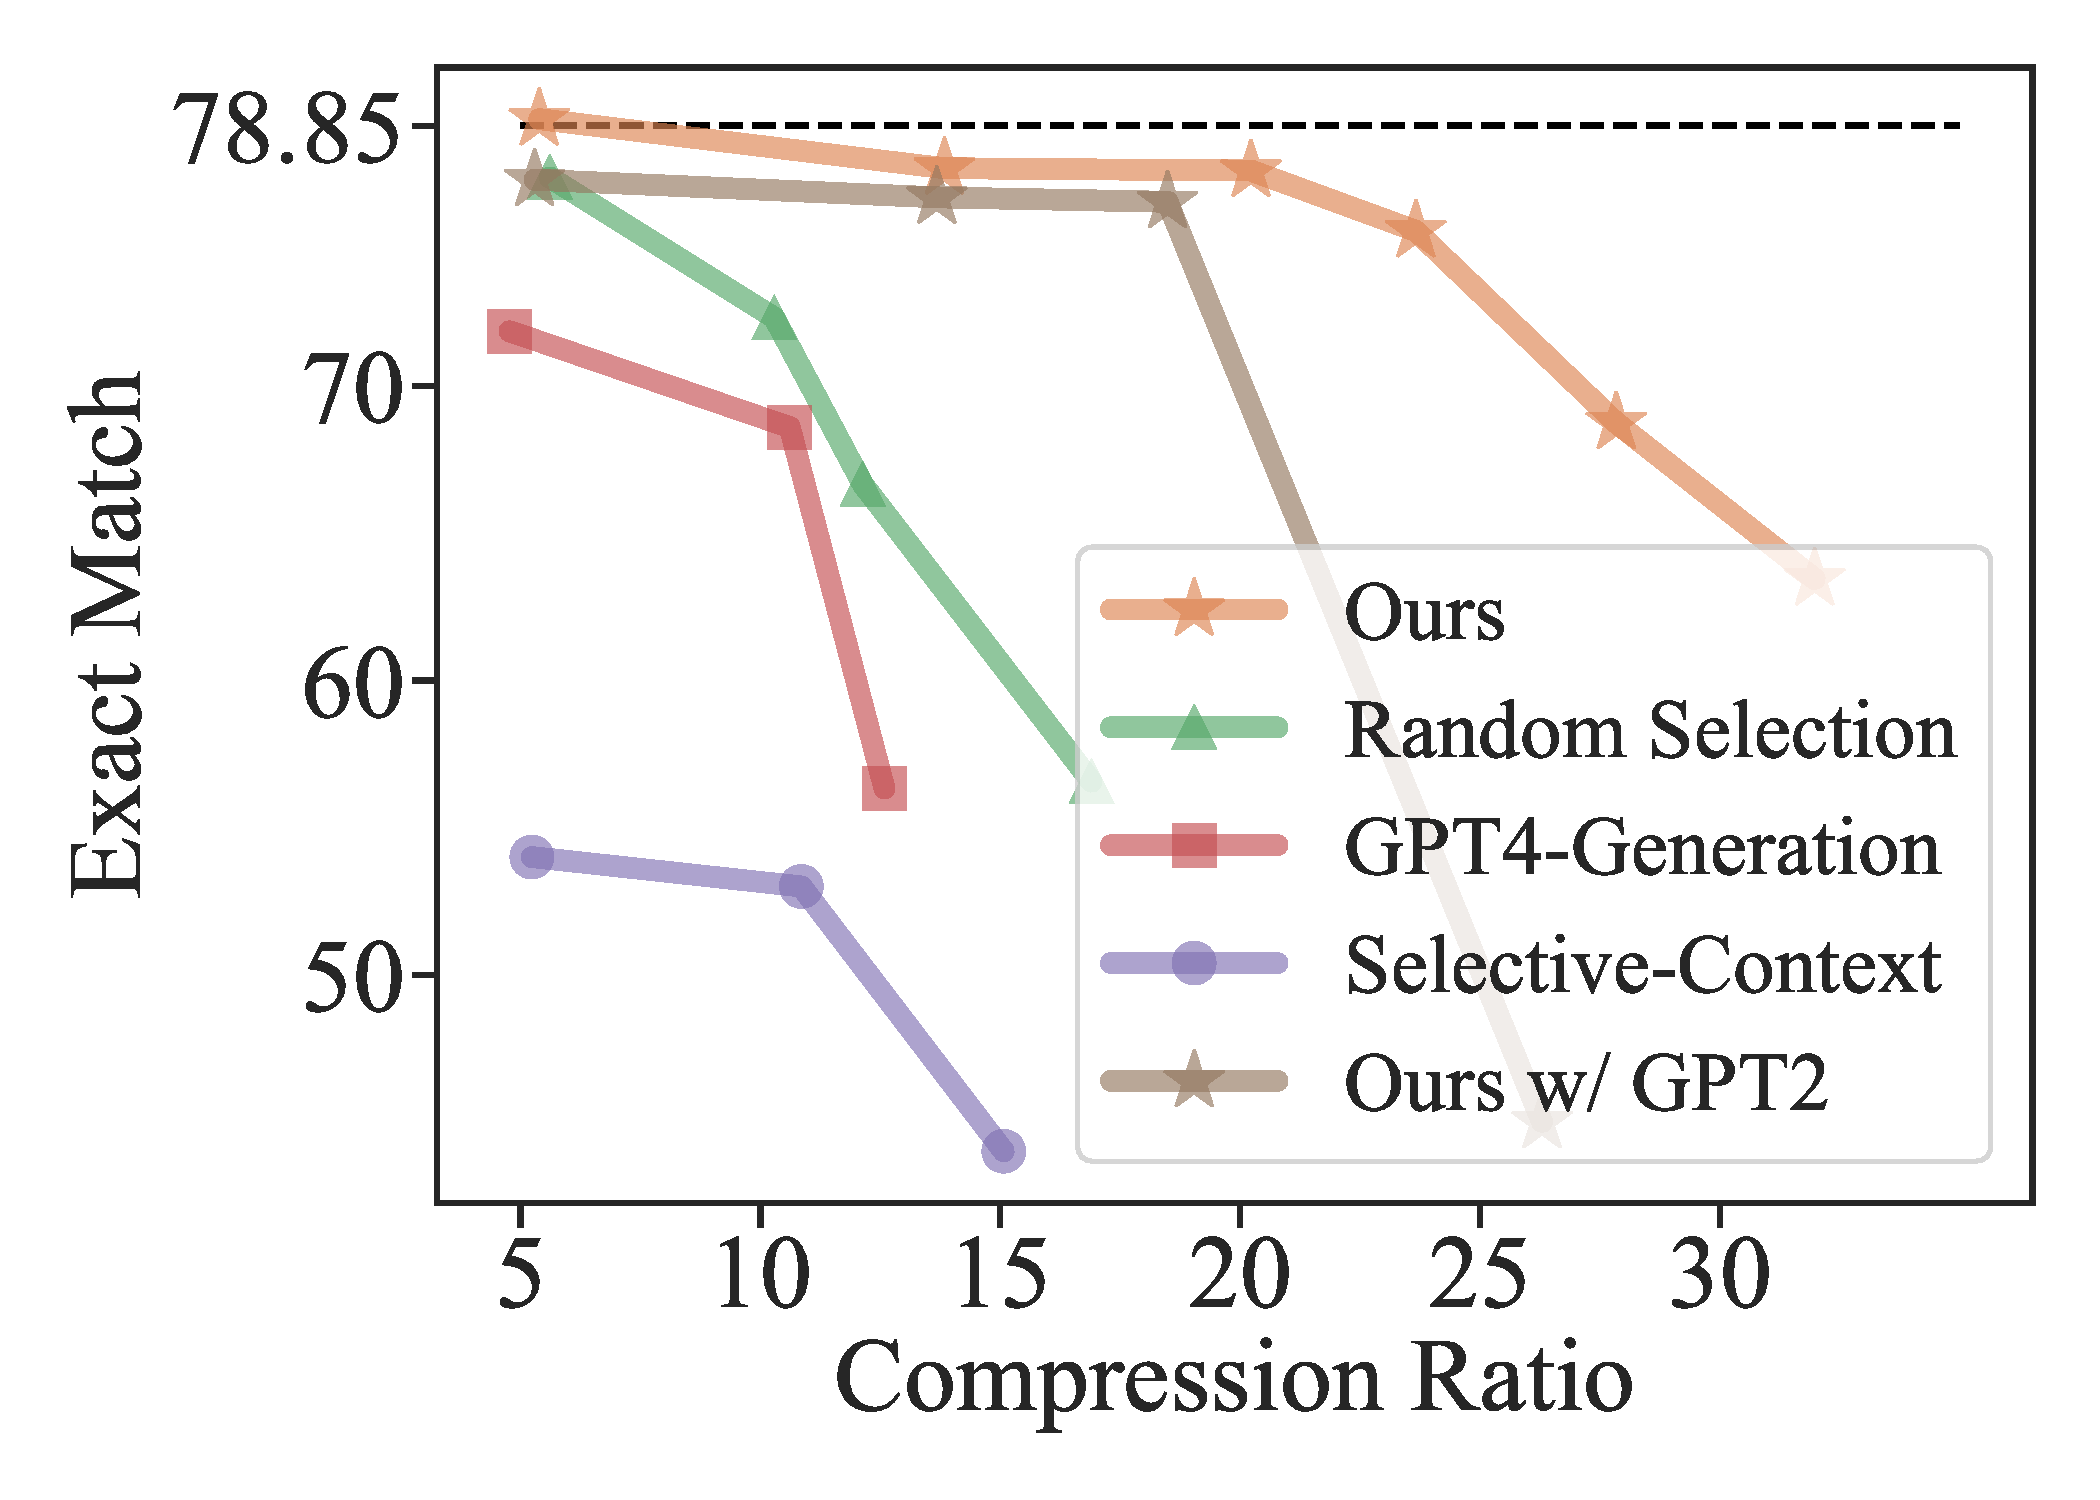
\includegraphics[width=\linewidth]{figures/compression_ratio_performance_gsm8k.pdf}
%     \caption{The performance of various prompt compression methods at different ratios ($1/\tau$) on GSM8K.}
%     \label{fig:big_compression_atio}
% \end{figure}

% \paragraph{Upperbound of Compression Ratio}
% As shown in Figure~\ref{fig:big_compression_atio}, we also conducted tests at higher compression ratios. It can be observed that as the compression ratio further increases, even our method experiences a noticeable performance drop around 25x-30x. In comparison with other methods, this performance drop is significantly shifted to the right, thanks to the Budget Controller and Iterative Token-level Prompt Compression, which enable our method to maintain the original prompt information even at more extreme compression ratios. The upper limit of the compression ratio for different prompts varies, depending on factors such as prompt length, task type, and the number of sentences.

\paragraph{The Generation Results of Compressed Prompt}
% case study
% generation length

Appendix~\ref{sec:cases_study} displays several compressed prompts along with following generation texts.
It is evident that the compressed prompts can still guide the generation of multi-step reasoning outcomes similar to the original ones. In contrast, prompts compressed using Selective-Context exhibit errors in reasoning logic. This highlights the effectiveness of our method in preserving crucial semantic information while retaining reasoning capabilities.

\begin{figure}[htb]
    \centering
    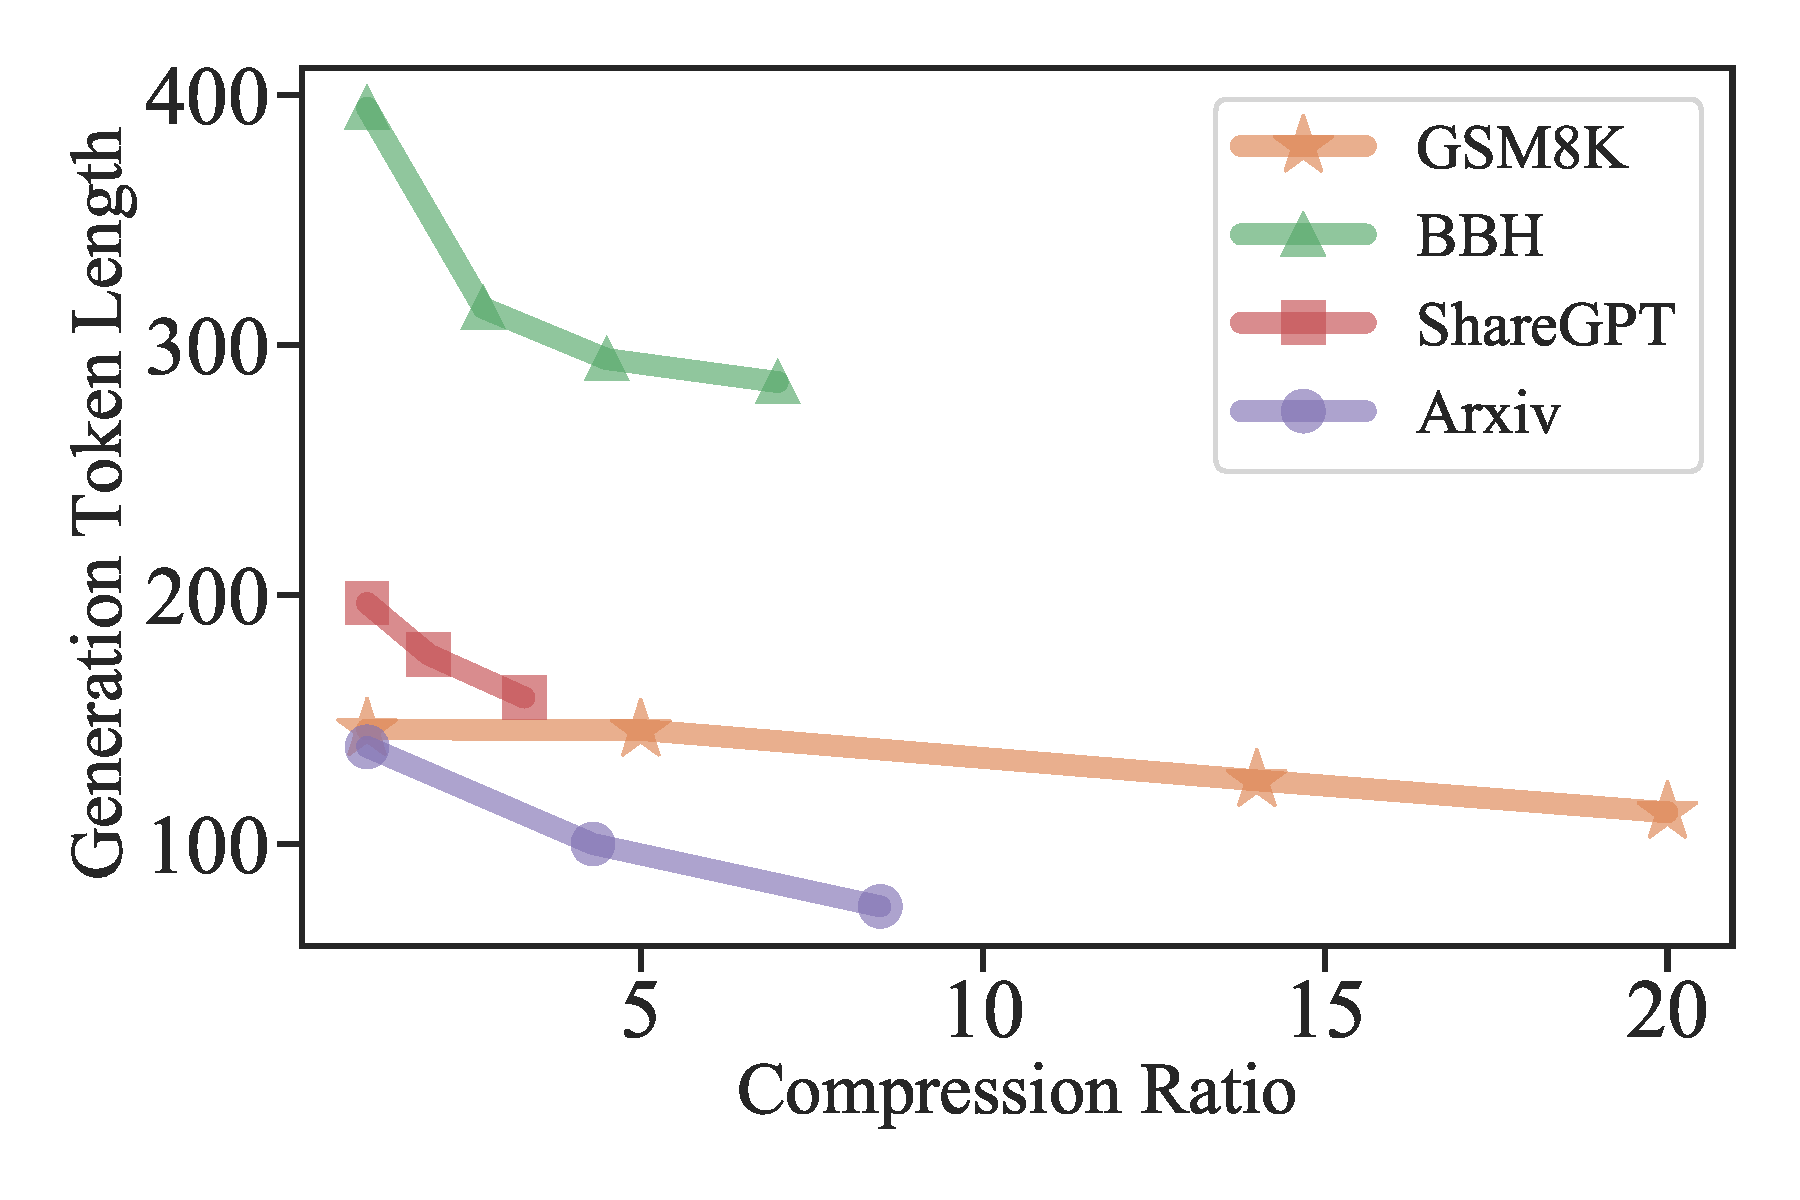
\includegraphics[width=\linewidth]{figures/compression_ratio_generation_length.pdf}
    \caption{The distribution of generated token lengths at varying compression ratios ($1/\tau$).}
    \label{fig:compression_ratio_vs_generation_length}
\end{figure}

As depicted in Figure~\ref{fig:compression_ratio_vs_generation_length}, we also analyze 
% the impact of prompt compression on the generated text length.
the relationship between the compression ratio and the length of the corresponding generated texts.
It can be observed that as the compression ratio increases, the text length produced by target LLMs tends to decrease, albeit with varying degrees across different datasets. This indicates that prompt compression not only saves computational resources in the input but also contributes to computational savings in the generation stage.


\paragraph{{Overhead of \sysname{}}}

% Using \sysname{} to compress prompts has a very small computation overhead. Next, we will explain this from two aspects: estimating the number of tokens involved in the computation and measuring end-to-end latency.
% \sysname{} only incurs a little computational overhead.
We explore two key factors to study the computation overhead of \sysname{}: the number of tokens involved in computation and the end-to-end latency.

The overall computation %load 
of our system is the sum of the % computation required for 
prompt compression and the %computation needed for 
following inference. % on the compressed prompt, which can be formulated as:
This can be formulated as:
\begin{equation}
    c = (L + kL/\tau + L/\tau) \cdot c_{\text{small}} + L/\tau \cdot c_{\text{LLMs}},
\end{equation}
where $c_{\text{small}}$ and $c_{\text{LLMs}}$ represent the per token computation load of the small LM and LLM, respectively.
$L$, $kL/\tau$, and $L/\tau$ 
are the numbers of token inferences for the budget controller, the perplexity calculation of tokens to compress in ITPC, and the conditioned perplexity calculation of compressed results in ITPC (using KV cache), respectively.
% are the numbers of token calculation corresponding to the budget controller, the perplexity calculation, and condition updating calculation after compressing, by using KV cache, in iterative token-level prompt compression, respectively. 
Assuming that the small LM has the same system optimizations as the LLMs, such as the use of FasterTransformer\footnote{https://github.com/NVIDIA/FasterTransformer} and quantization techniques, we can estimate the ratio between $c_{\text{small}}$ and $c_{\text{LLMs}}$ based on model parameters: %, resulting in
$c_{\text{small}} \approx 7/175c_{\text{LLMs}} = 1/25c_{\text{LLMs}}$. When $\tau=5$, we have $c \approx 0.264 \cdot Lc_{\text{LLMs}} \approx 1/4 \cdot Lc_{\text{LLMs}}$.
% Therefore, it is estimated that when the prompt compression rate is 5x, we can achieve nearly 4x savings in computational resources.
That is, we can achieve nearly 4x savings in computational resources when using the smaller LM with a prompt compression rate of 5x.

\begin{table}[htb]
    \centering
	\setlength{\tabcolsep}{0.5mm}
	\scalebox{0.8}{
    \begin{tabular}{lcccc}
    \toprule
        $1/\tau$ & 1x & 2x & 5x & 10x \\
         \midrule
        End-to-End w/o LLMLingua & 8.6 & - & - & -\\
        End-to-End w/ LLMLingua & - & 4.9(1.7x) & 2.3(3.3x) & 1.3(5.7x)\\
        LLMLingua  & - & 0.8 & 0.3 & 0.2 \\
        \bottomrule
    \end{tabular}
    }
    \caption{Latency (s) comparison on GSM8K.}
    \label{tab:latency}
\end{table}
Table~\ref{tab:latency} shows the end-to-end latency of different systems on a V100-32G GPU with a compression rate from 1x to 10x.
% in different processing and compression ratios 
We can see that LLMLingua has a relatively small computation overhead and can achieve a speedup ranging from 1.7x to 5.7x.

 
\paragraph{Recovering the Compressed Prompt using LLMs}
% \paragraph{The Reasoning Information in Compressed Prompt}
Appendix~\ref{sec:recover_cases} shows some examples restored from the compressed prompts by using GPT-4\footnote{{An intriguing observation is that GPT-3.5-Turbo struggles to reconstruct compressed prompts, while GPT-4 has demonstrated an ability to do so. This contrast in performance could suggest that recovering compressed prompts is an emergent ability that arises in more advanced language models.}}.
It is evident that LLMs can effectively comprehend the semantic information in the compressed prompts, even if it might be challenging for humans.
Additionally, we notice that how much information GPT-4 can recover depends on the compression ratio and the small language model we use.
For instance, in Figure~\ref{fig:prompt_recovered}, the prompt compressed using Alpaca-7B is restored to its complete 9-step reasoning process, while in Figure~\ref{fig:prompt_recovered_gpt2}, the prompt compressed with GPT2-Alpaca can only be restored to a 7-step reasoning process, with some calculation errors.
%with some errors shown up in calculations.
% \red{However, an interesting phenomenon is that GPT-3.5-Turbo struggles to recover compressed prompts, which might be a form of emergent ability.}


% 压缩率 曲线 -> GSM8K 更高压缩率
% 对generation 结果的分析
% 对multi-step 的分析

% 对prompt compression,还会对generation 过程的推理长度也相应的的减少,例如geometric_shapes
% 经济开销计算
% 两张图
% 1. Difference \tau v.s. performance in GSM8K
% 2. Difference \tau v.s. generation \tau


% \subsection{Discussion}



\paragraph{Compare with Generation-based Methods}
% We have opted not to use generated-based methods in this study for three main reasons.
We do not develop our approach based on LLM generation primarily for three reasons:
i) The content and length of the generated text are uncontrollable. Uncontrollable length requires more iterations to satisfy the constraint of the compression ratio.
Uncontrollable content leads to low overlap between the generated text and the original prompt, particularly for complex prompts with multi-step inference, which may lose significant amounts of reasoning paths or even generate completely unrelated demonstrations.
ii) The computational cost is high. Small language models struggle to handle such complex tasks, and using models like GPT-4 for compression would further increase computational overhead. Moreover, even powerful generation models like GPT-4 struggle to retain effective information from prompts as shown in Table~\ref{tab:main_results}.
iii) The compressed prompts obtained from generation models are complete and continuous sentences, usually resulting in a lower compression ratio compared to our coarse-to-fine method.
% Nonetheless, owing to the necessity for linguistic completeness, our method's theoretical compression upper limit is lower compared to generation-based approaches.


\paragraph{Compare with Prompt Engineering methods}

Our method is orthogonal to Prompt Engineering methods, such as prompt retrieval and prompt ordering. Our work focuses on compressing well-designed prompts, and it performs well on complex and fine-tuned prompts like GSM8K. Moreover, the perplexity-based demonstration filtering method used in our budget controller can also be applied to scenarios such as prompt retrieval. This demonstrates the compatibility and adaptability of our approach in various LLMs settings.

% \paragraph{Economic Cost}
% \begin{table}[ht]
    \centering
	\setlength{\tabcolsep}{0.5mm}
	% \scalebox{0.8}{
     \resizebox{0.7\columnwidth}{!}{
    \begin{tabular}{lcccc}
    \toprule
         & GSM8K & BBH & ShareGPT & Arxiv \\
         \midrule
        Original & 5.2 & 12.8 & 0.7 & 1.3 \\
        Ours & 0.5 & 4.8 & 0.3 & 0.2 \\
        \bottomrule
    \end{tabular}
    }
    % }
    \caption{The inference costs(\$) for various datasets using GPT-3.5-Turbo.}
    \label{tab:cost}
\end{table}

% Table~\ref{tab:cost} presents the estimated inference costs for different datasets, based on gpt-3.5-Turbo's pricing structure. Our method demonstrates substantial savings in computational resources and monetary expenses, with cost reductions of \$4.7, \$8.0, \$0.4, and \$0.8 observed in the GSM8K, BBH, ShareGPT, and Arxiv datasets, respectively.
% \paragraph{longer prompt}

% 不选generation 方式的原因讨论
% 与Prompt Order, Prompt Retrieval 等技术的关系
% 增加部分prompt 是否会提升performance


